\chapter{Implementazione}
%‘‘’’
Sia per la realizzazione del front end che del discovery service ho utilizzato TypeScript, sfruttando le funzionalità offerte dalla libreria JavaScript di Radix. 

Per velocizzare lo sviluppo del discovery service, ho usato come base di partenza un server realizzato con TypeScript e WebPack. Ad esso ho aggiunto il codice per la connessione ad un database locale MongoDB, per tenere traccia di tutte le informazioni relative ai bootleg. Essendo a tutti gli effetti un server, per comunicare con il Discovery Service vengono utilizzate delle normali richieste http, costruite utilizzando la libreria axios.

Per il front end invece ho utilizzato il framework Vue.js, in quanto permette di realizzare un interfaccia utente in maniera piuttosto semplice, e inoltre consente di mantenere le astrazioni di Radix (Atom, Transazioni, ecc.) separate dal codice HTML.

Come già accennato in precedenza, attualmente non è stata ancora attivata la rete pubblica di Radix, dunque per sviluppare applicazioni è necessario simulare la rete sulla propria macchina. Per farlo, è disponibile un emulatore da eseguire in locale, attraverso un'immagine Docker. Una volta lanciato l'Emulator, sarà disponibile collegarsi ad una rete Radix ed eseguire correttamente l'applicazione. Il modo in cui eseguire il Betanet Emulator sulla propria macchina è spiegato nella documentazione di Radix: [https://docs.radixdlt.com/kb/develop/betanet-emulator](https://docs.radixdlt.com/kb/develop/betanet-emulator). 

Sempre nella documentazione Radix è possibile consultare diversi esempi di codice che sono stati fondamentali durante l'implementazione del progetto.

\section{Utilizzo dei Token}

Per effettuare i pagamenti dei bootleg all'interno dell'applicazione, viene usato il token BTLG. Il discovery service definisce il token BTLG al suo primo avvio come un token multi-issuance. Nel momento in cui un utente crea una nuova identity, il frontend invia una richiesta al discovery service per ricevere una somma iniziale di token BTLG token. In sostanza, il Discovery Service prende il posto del Faucet, ovvero un account particolare che ha lo scopo di inviare dei token nativi di test. 

Il Discovery Service ha anche il compito di definire un Token univoco per ciascun bootleg nel momento della sua creazione. Il possesso di questo Token da parte di un utente è ciò che indica al sistema che tale utente ha acquistato il relativo bootleg, e pertanto è autorizzato a visualizzarlo.

\section{Gestione dell'identity}

La libreria Radix offre delle funzionalità per la gestione delle identity all'interno di un'applicazione. La funzione `encryptKey`, date in input un'identity e una password, cifra la prima producendo in output un oggetto JSON detto anche \textit{keystore}. L'identity viene decifrata usando la funzione `decryptKey`, fornendo in input il keystore e la password utilizzata per produrlo.

Per la gestione dell'identity all'interno dell'applicazione sono disponibili due diverse opzioni:
\begin{itemize}
    \item Generare una nuova identity locale.
    \item Usare un'identity remota.
\end{itemize}

\begin{figure}[H]
  \centering
  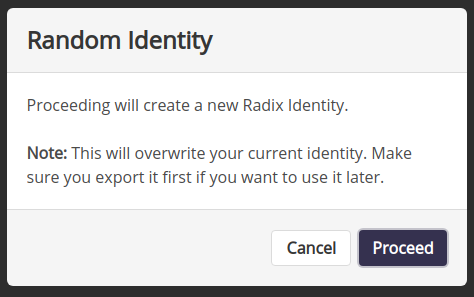
\includegraphics[width=0.75\textwidth]{images/application/create_random.png}
  \caption{Creazione di una nuova identity locale}
  \label{fig:trex}
\end{figure}

Quando l'utente genera una nuova identity locale, questa viene automaticamente cifrata con una password di default e il keystore viene salvato nella memoria del browser utilizzando la proprietà `Window.localStorage`. In questo modo, l'identity viene recuperata all'avvio successivo del browser. Quando l'utente genera una nuova identity locale, quella precedente viene sovrascritta. Tuttavia, l'applicazione offre anche la possibilità di \textit{esportare} la propria identity: Facendo export l'applicazione chiede all'utente di inserire una password per cifrare la chiave, e mostra il keystore JSON prodotto. L'utente può così salvare il contenuto del keystore all'interno di un file, che potrà così essere recuperato in un secondo momento. Con la funzione *import* infatti, l'utente inserisce il *keystore* e la password inserita in precedenza, e l'identity che ha esportato viene così importata dentro l'applicazione.

\begin{figure}[H]
  \centering
  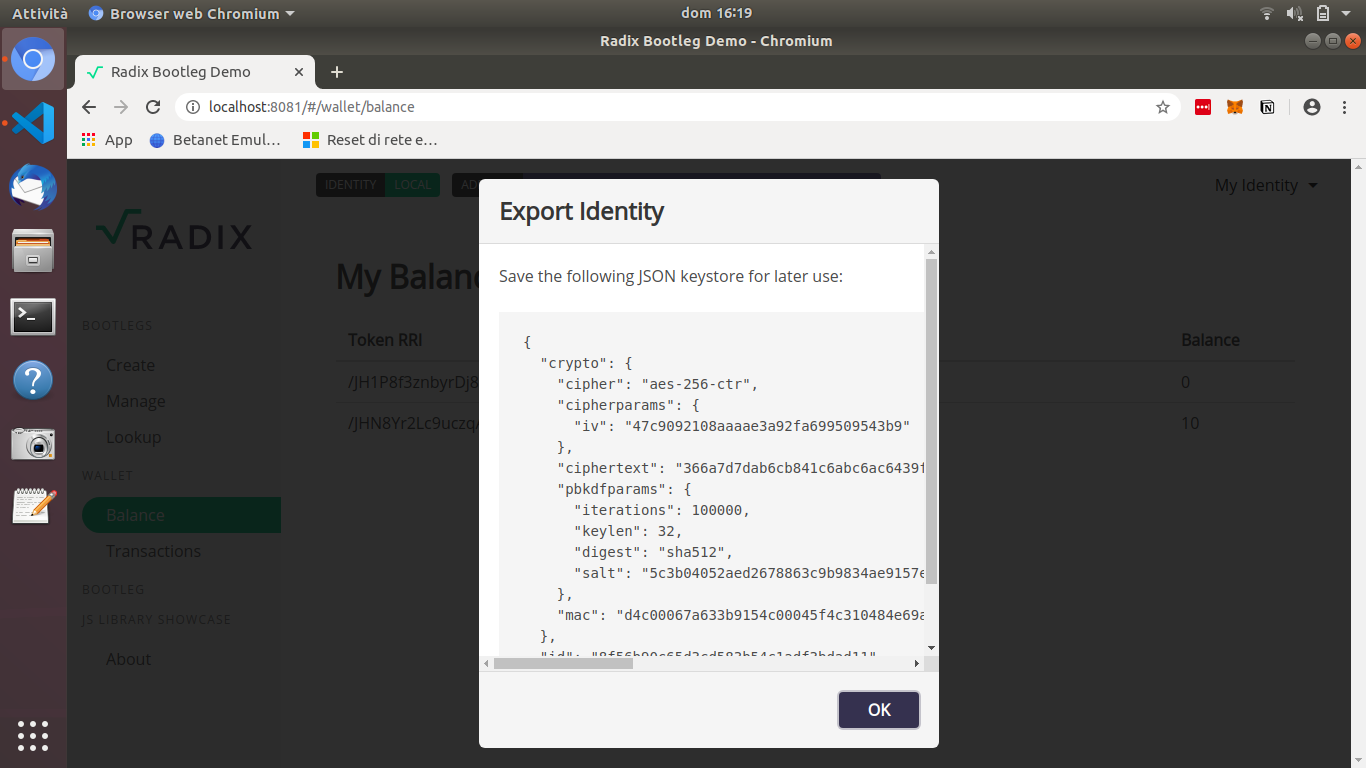
\includegraphics[width=\linewidth]{images/application/save-keystore.png}
  \caption{Esportazione di un'identity locale}
  \label{fig:trex}
\end{figure}

Usando un'identity remota invece, l'applicazione userà la chiave privata salvata nel Radix Wallet dell'utente, che pertanto non necessita di essere salvata nel browser. In questo caso, l'applicazione invia una richiesta al Radix Wallet. Una volta che l'utente accetta la richiesta, l'applicazione potrà usare la chiave privata mantenuta nel Wallet per firmare atom per conto dell'utente. 

\section{Creazione di un bootleg}

Per creare un bootleg, è necessario inserire:
\begin{itemize}
    \item Simbolo usato per il token;
    \item Titolo del bootleg;
    \item Indirizzo dell'artista;
    \item Prezzo del bootleg;
    \item Url del bootleg (Per semplicità sono stati utilizzati dei link di video su YouTube);
\end{itemize}

Quando l'utente da la conferma, questi vengono inviati al server (Discovery Service), che provvederà a creare il token per il bootleg e salverà tutti i dati inviati dall'utente sul database, insieme all'identificativo del token appena creato, ed agli indirizzi di bootlegger e artista. Terminato l'inserimento, il Discovery Service invierà all'utente l'identificativo del token come conferma.

\section{Acquisto di un bootleg}

L'applicazione recupera la lista dei bootleg inseriti sul database inviando una richiesta al Discovery Service, che esegue una query e recupera tutti i dati dei bootleg (ad eccezione dell'url del video), e li invia al frontend.

Per ciascun bootleg nella lista, il front end verifica se sono presenti nell'account dell'utente, e in caso contrario mostra un pulsante ‘‘Buy’’.

Quando un utente acquista un bootleg, l'applicazione verifica che il suo account possieda un ammontare sufficiente di BTLG. Se si, il pagamento viene inviato al discovery service, insieme ai dati del bootleg da acquistare. Il Discovery Service può così dividere il pagamento in parti uguali tra artista, bootlegger ed eventuali franchisor.

Una volta che il pagamento è stato diviso tra i vari destinatari, il discovery service procede con l'invio del token all'utente ed inserisce quest'ultimo nella lista dei franchisor per quel token, aggiornando i dati sul database. In questo modo, quando verrà effettuato un nuovo acquisto del bootleg, l'utente riceverà una percentuale del pagamento come franchisor. 

\section{Visualizzazione del bootleg}

Una volta che l'utente possiede il token, nella lista dei bootleg compare il pulsante ‘‘Watch’’ di fianco al bootleg, che consente all'utente di visualizzare il bootleg. Dal momento che il front-end non possiede di per se l'url del video, deve richiederlo al Discovery Service. Il modo in cui il frontend richiede ed ottiene il link al contenuto del bootleg si basa su uno schema challenge-response. 

Cliccando su ‘‘Watch’’ il front end invia una richiesta al Discovery service per il link al bootleg.Quando il DS riceve questa richiesta, crea una \textit{challenge} casuale, la salva nel database insieme ad un attributo boolean \textit{consumed}, inizialmente settato a ‘‘false’’, per indicare che la challenge non è stata ancora utilizzata per accedere ad un bootleg. 

Quando il frontend riceve la challenge dal Discovery Service, crea un nuovo Payload Atom contenente la challenge, firma questo Atom con la propria identity e lo invia al Discovery Service con una richiesta http insieme all'URI del token del bootleg da visualizzare.

Una volta che il Discovery Service riceve anche questa richiesta:
\begin{enumerate}
    \item Estrae l'atom dalla richiesta e verifica la validità della firma dell'atom, cioè controlla se è stata prodotta dall'account che ha creato l'atom. Se la firma viene verificata con successo, il DS procede con la verifica della challenge.
    \item Verifica la validità della challenge: il DS estrae la challenge dal payload dell'atom, ed esegue una query sul database per trovare la challenge ricevuta. Se non viene trovata la challenge, oppure viene trovata ma l'attributo ‘‘consumed’’ ha valore ‘‘true’’ (dunque è già stata utilizzata), la challenge non viene considerata valida e il DS restituisce un errore al frontend. Altrimenti, aggiorna il valore di ‘‘consumed’’ a true sul database e prosegue al passo successivo.
    \item Verifica il possesso del bootleg: Il DS controlla il saldo dell'account dell'utente che ha inviato la richiesta e verifica se è presente il token del bootleg richiesto. Se il token è presente, allora il DS recupera il link del video dal database e lo invia come risposta al frontend.
\end{enumerate}

Una volta che il frontend riceve il link del bootleg, mostra all'utente il video YouTube attraverso un elemento `<iframe>`.